\documentclass[]{book}
\usepackage{lmodern}
\usepackage{amssymb,amsmath}
\usepackage{ifxetex,ifluatex}
\usepackage{fixltx2e} % provides \textsubscript
\ifnum 0\ifxetex 1\fi\ifluatex 1\fi=0 % if pdftex
  \usepackage[T1]{fontenc}
  \usepackage[utf8]{inputenc}
\else % if luatex or xelatex
  \ifxetex
    \usepackage{mathspec}
  \else
    \usepackage{fontspec}
  \fi
  \defaultfontfeatures{Ligatures=TeX,Scale=MatchLowercase}
\fi
% use upquote if available, for straight quotes in verbatim environments
\IfFileExists{upquote.sty}{\usepackage{upquote}}{}
% use microtype if available
\IfFileExists{microtype.sty}{%
\usepackage{microtype}
\UseMicrotypeSet[protrusion]{basicmath} % disable protrusion for tt fonts
}{}
\usepackage[margin=1in]{geometry}
\usepackage{hyperref}
\hypersetup{unicode=true,
            pdftitle={The R in Spark},
            pdfauthor={Javier Luraschi},
            pdfborder={0 0 0},
            breaklinks=true}
\urlstyle{same}  % don't use monospace font for urls
\usepackage{natbib}
\bibliographystyle{apalike}
\usepackage{color}
\usepackage{fancyvrb}
\newcommand{\VerbBar}{|}
\newcommand{\VERB}{\Verb[commandchars=\\\{\}]}
\DefineVerbatimEnvironment{Highlighting}{Verbatim}{commandchars=\\\{\}}
% Add ',fontsize=\small' for more characters per line
\usepackage{framed}
\definecolor{shadecolor}{RGB}{248,248,248}
\newenvironment{Shaded}{\begin{snugshade}}{\end{snugshade}}
\newcommand{\AlertTok}[1]{\textcolor[rgb]{0.94,0.16,0.16}{#1}}
\newcommand{\AnnotationTok}[1]{\textcolor[rgb]{0.56,0.35,0.01}{\textbf{\textit{#1}}}}
\newcommand{\AttributeTok}[1]{\textcolor[rgb]{0.77,0.63,0.00}{#1}}
\newcommand{\BaseNTok}[1]{\textcolor[rgb]{0.00,0.00,0.81}{#1}}
\newcommand{\BuiltInTok}[1]{#1}
\newcommand{\CharTok}[1]{\textcolor[rgb]{0.31,0.60,0.02}{#1}}
\newcommand{\CommentTok}[1]{\textcolor[rgb]{0.56,0.35,0.01}{\textit{#1}}}
\newcommand{\CommentVarTok}[1]{\textcolor[rgb]{0.56,0.35,0.01}{\textbf{\textit{#1}}}}
\newcommand{\ConstantTok}[1]{\textcolor[rgb]{0.00,0.00,0.00}{#1}}
\newcommand{\ControlFlowTok}[1]{\textcolor[rgb]{0.13,0.29,0.53}{\textbf{#1}}}
\newcommand{\DataTypeTok}[1]{\textcolor[rgb]{0.13,0.29,0.53}{#1}}
\newcommand{\DecValTok}[1]{\textcolor[rgb]{0.00,0.00,0.81}{#1}}
\newcommand{\DocumentationTok}[1]{\textcolor[rgb]{0.56,0.35,0.01}{\textbf{\textit{#1}}}}
\newcommand{\ErrorTok}[1]{\textcolor[rgb]{0.64,0.00,0.00}{\textbf{#1}}}
\newcommand{\ExtensionTok}[1]{#1}
\newcommand{\FloatTok}[1]{\textcolor[rgb]{0.00,0.00,0.81}{#1}}
\newcommand{\FunctionTok}[1]{\textcolor[rgb]{0.00,0.00,0.00}{#1}}
\newcommand{\ImportTok}[1]{#1}
\newcommand{\InformationTok}[1]{\textcolor[rgb]{0.56,0.35,0.01}{\textbf{\textit{#1}}}}
\newcommand{\KeywordTok}[1]{\textcolor[rgb]{0.13,0.29,0.53}{\textbf{#1}}}
\newcommand{\NormalTok}[1]{#1}
\newcommand{\OperatorTok}[1]{\textcolor[rgb]{0.81,0.36,0.00}{\textbf{#1}}}
\newcommand{\OtherTok}[1]{\textcolor[rgb]{0.56,0.35,0.01}{#1}}
\newcommand{\PreprocessorTok}[1]{\textcolor[rgb]{0.56,0.35,0.01}{\textit{#1}}}
\newcommand{\RegionMarkerTok}[1]{#1}
\newcommand{\SpecialCharTok}[1]{\textcolor[rgb]{0.00,0.00,0.00}{#1}}
\newcommand{\SpecialStringTok}[1]{\textcolor[rgb]{0.31,0.60,0.02}{#1}}
\newcommand{\StringTok}[1]{\textcolor[rgb]{0.31,0.60,0.02}{#1}}
\newcommand{\VariableTok}[1]{\textcolor[rgb]{0.00,0.00,0.00}{#1}}
\newcommand{\VerbatimStringTok}[1]{\textcolor[rgb]{0.31,0.60,0.02}{#1}}
\newcommand{\WarningTok}[1]{\textcolor[rgb]{0.56,0.35,0.01}{\textbf{\textit{#1}}}}
\usepackage{longtable,booktabs}
\usepackage{graphicx,grffile}
\makeatletter
\def\maxwidth{\ifdim\Gin@nat@width>\linewidth\linewidth\else\Gin@nat@width\fi}
\def\maxheight{\ifdim\Gin@nat@height>\textheight\textheight\else\Gin@nat@height\fi}
\makeatother
% Scale images if necessary, so that they will not overflow the page
% margins by default, and it is still possible to overwrite the defaults
% using explicit options in \includegraphics[width, height, ...]{}
\setkeys{Gin}{width=\maxwidth,height=\maxheight,keepaspectratio}
\IfFileExists{parskip.sty}{%
\usepackage{parskip}
}{% else
\setlength{\parindent}{0pt}
\setlength{\parskip}{6pt plus 2pt minus 1pt}
}
\setlength{\emergencystretch}{3em}  % prevent overfull lines
\providecommand{\tightlist}{%
  \setlength{\itemsep}{0pt}\setlength{\parskip}{0pt}}
\setcounter{secnumdepth}{5}
% Redefines (sub)paragraphs to behave more like sections
\ifx\paragraph\undefined\else
\let\oldparagraph\paragraph
\renewcommand{\paragraph}[1]{\oldparagraph{#1}\mbox{}}
\fi
\ifx\subparagraph\undefined\else
\let\oldsubparagraph\subparagraph
\renewcommand{\subparagraph}[1]{\oldsubparagraph{#1}\mbox{}}
\fi

%%% Use protect on footnotes to avoid problems with footnotes in titles
\let\rmarkdownfootnote\footnote%
\def\footnote{\protect\rmarkdownfootnote}

%%% Change title format to be more compact
\usepackage{titling}

% Create subtitle command for use in maketitle
\newcommand{\subtitle}[1]{
  \posttitle{
    \begin{center}\large#1\end{center}
    }
}

\setlength{\droptitle}{-2em}
  \title{The R in Spark}
  \pretitle{\vspace{\droptitle}\centering\huge}
  \posttitle{\par}
  \author{Javier Luraschi}
  \preauthor{\centering\large\emph}
  \postauthor{\par}
  \predate{\centering\large\emph}
  \postdate{\par}
  \date{2018-04-19}

\usepackage{booktabs}
\usepackage{amsthm}
\makeatletter
\def\thm@space@setup{%
  \thm@preskip=8pt plus 2pt minus 4pt
  \thm@postskip=\thm@preskip
}
\makeatother

\usepackage{amsthm}
\newtheorem{theorem}{Theorem}[chapter]
\newtheorem{lemma}{Lemma}[chapter]
\theoremstyle{definition}
\newtheorem{definition}{Definition}[chapter]
\newtheorem{corollary}{Corollary}[chapter]
\newtheorem{proposition}{Proposition}[chapter]
\theoremstyle{definition}
\newtheorem{example}{Example}[chapter]
\theoremstyle{definition}
\newtheorem{exercise}{Exercise}[chapter]
\theoremstyle{remark}
\newtheorem*{remark}{Remark}
\newtheorem*{solution}{Solution}
\begin{document}
\maketitle

{
\setcounter{tocdepth}{1}
\tableofcontents
}
\hypertarget{the-r-in-spark}{%
\chapter*{The R in Spark}\label{the-r-in-spark}}
\addcontentsline{toc}{chapter}{The R in Spark}

In this book you will learn Apache Spark using R. The book intends to
take someone unfamiliar with Spark or R and help them become
intermediate users by teaching a set of tools, skills and practices
applicable to data science.

This work is licensed under the
\href{http://creativecommons.org/licenses/by-nc-nd/3.0/us/}{Creative
Commons Attribution-NonCommercial-NoDerivs 3.0} United States License.

\hypertarget{intro}{%
\chapter{Introduction}\label{intro}}

This chapters covers the historical background that lead to the
development of Spark, introduces R in the context of Spark and
\texttt{sparklyr} as a project bridging Spark and R.

\hypertarget{background}{%
\section{Background}\label{background}}

\href{https://en.wikipedia.org/wiki/Information_technology}{Humans have
been storing, retrieving, manipulating, and communicating information
since the Sumerians in Mesopotamia developed writing in about 3000 BC}.
Based on the storage and processing technologies employed, it is
possible to distinguish four distinct phases development: pre-mechanical
(3000 BC -- 1450 AD), mechanical (1450--1840), electromechanical
(1840--1940), and electronic (1940--present).

\href{https://en.wikipedia.org/wiki/Information_Age}{As humanity moves
from traditional industries to an economy based on information
technology} our footprint of digital information has kept growing at
\href{http://documents.worldbank.org/curated/en/896971468194972881/310436360_201602630200201/additional/102725-PUB-Replacement-PUBLIC.pdf}{exponential
rates} (see Section \ref{storage-capacity}):

\begin{figure}
\centering
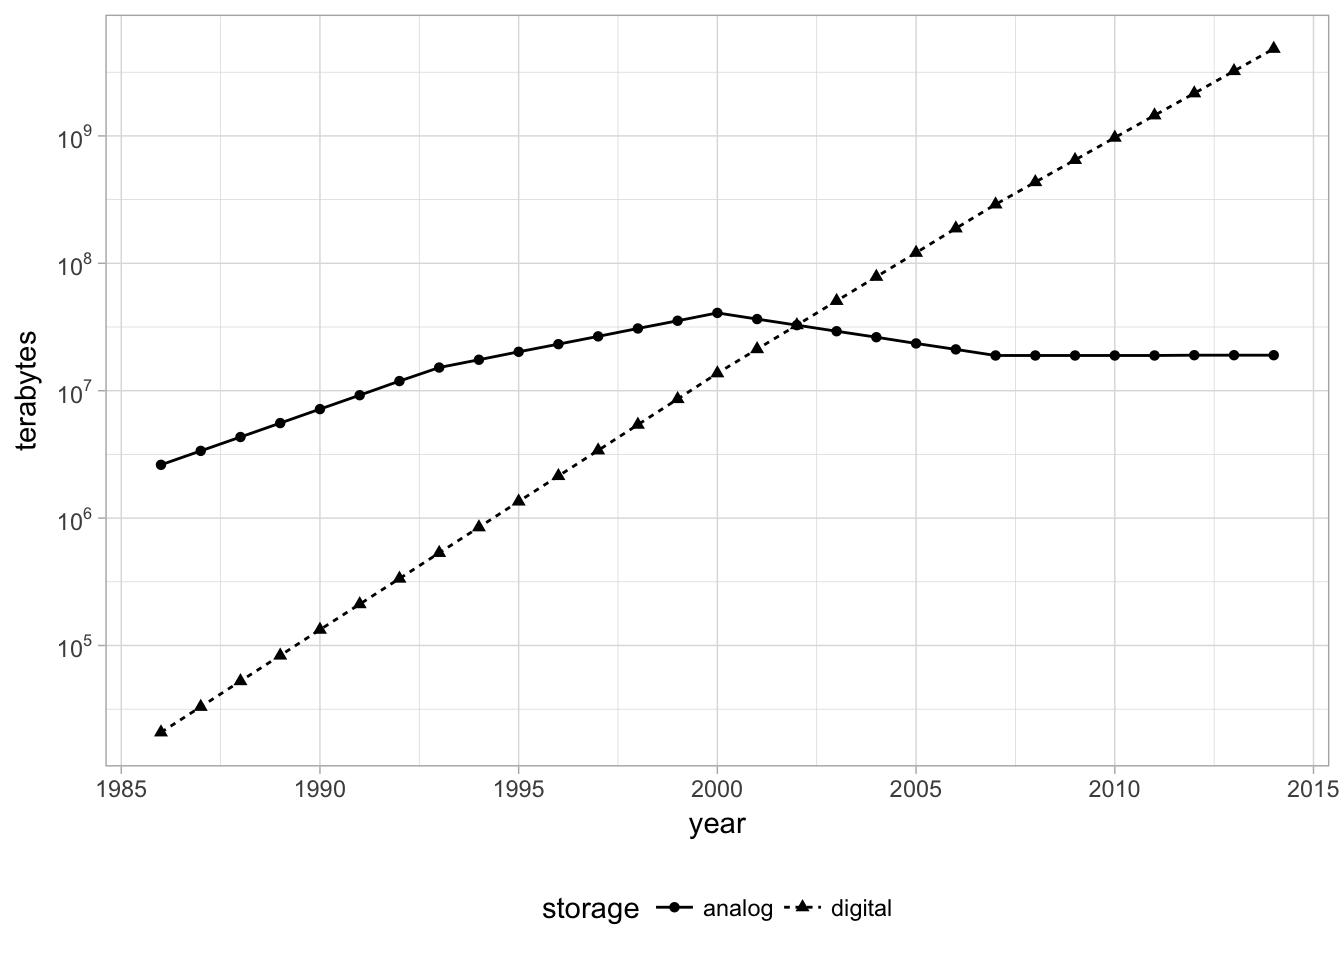
\includegraphics{the-r-in-spark_files/figure-latex/unnamed-chunk-1-1.pdf}
\caption{\label{fig:unnamed-chunk-1}World's capacity to store information.}
\end{figure}

With the ambition to provide a searchable tool to all this new digital
information, many companies attempted to provide such functionality with
what we now know as web search or search engines. Managing information
at this scale was a challenging problem that companies had to tackle
from the very beginning. Given the vast amount of digital information,
search engiens were unble to store all the web page information required
to support web searches in a single computer. This meant that they had
to split information across many machines, which was accomlished by
splitting this data and storing it as many files across many machines,
this approach became known as the Google File System from a research
paper published in 2003 by Google which has served for others to build
on.

One year later, in 2004, Google published a new paper describing how to
perform operations across the Google File System, this approach came to
be known as \textbf{MapReduce}. As you would expect, there are two
operations in MapReduce: Map and Reduce. We can think of the mapping
operation as a way to transform each file into a new file and, reuduce
as a way of combining two files into a new one. It happens to be the
case that using these two operations is sufficient to perform
interesting operations; for instance, MapReduce can be used to rank web
pages efficietly across a cluster of machines.

Since the papers were released by Google, a team in Yahoo worked on
implementing the Google File System and MapReduce as free open source
projects. This project was released in 2006 as \textbf{Hadoop} and the
Google File System became implemented as the Hadoop File System, or HDFS
for short. The Hadoop project made distributed file-based computing
accessible to many users and organizations.

While Hadoop provided support to perform map/reduce operations over a
distributed file system, it still required each map/reduce operation to
be written with code every time a data analysys was run. The
\textbf{Hive} project, released in 2008 by Facebook, brought Structured
Query Language (SQL) support to Hadoop. This meant that data analysis
could now be performed at large-scale without the need to write code for
each map/reduce operation, but instead, one could write generic data
analysis statements that are much easier to understand and write.

\hypertarget{spark}{%
\section{Spark}\label{spark}}

While Hadoop with Hive was a powerful tool, it was still working over a
distributed file system and was dependent on map/reduce operations. This
meant that it was running using disk drives which tend to be
significantly slower than using a computer's memory. In 2009, the
\textbf{Apache Spark} projects starts in Berkeley to improve over
Hadoop. Specifically, by making use of memory (instead of disk drives)
and by providing a richer set of verbs beyond map/reduce, this allowed
it to be much faster and generic than its predecessor. For instance, one
can
\href{https://databricks.com/blog/2014/11/05/spark-officially-sets-a-new-record-in-large-scale-sorting.html}{sort
100TB of data in 72min and 2100 computers using Hadoop, but only 206
computers in 23min using Spark}. Spark was build using the Scala
programming language, but interfaces to other programming languages are
also provided today. Spark was released as an open source project in
2010 with the scope of the project defined as follows:

\begin{quote}
``Apache Spark is a fast and general engine for large-scale data
processing.''

--- \href{http://spark.apache.org/}{spark.apache.org}
\end{quote}

meaning that Spark is a tool designed to support:

\begin{itemize}
\tightlist
\item
  \textbf{Data Processing}: Data processing is the collection and
  manipulation of items of data to produce meaningful information
  \citep{data-processing}.
\item
  \textbf{Large-Scale}: What \emph{large} means is hard to quantify, but
  one can interpret this as cluster-scale instead, which represents a
  set of connected computers that work together.
\item
  \textbf{General}: Spark optimizes and executes parallel generic code,
  as in, there is no restriction as to what type of code one can write
  in Spark.
\item
  \textbf{Fast}: Spark is much faster than its predecessor by making
  efficient use of memory to speed data access while running algorithms
  at scale.
\end{itemize}

Spark is good at tackling large-scale data processing problems, this
usually known as \textbf{big data}
(\href{https://en.wikipedia.org/wiki/big_data}{data sets that are more
voluminous and complex that traditional ones}, but also is good at
tackling large-scale computation problems, known as \textbf{big compute}
(\href{https://www.nimbix.net/glossary/big-compute/}{tools and
approaches using a large amount of CPU and memory resources in a
coordinated way}). There is a third problem space where data nor compute
are necessarily large scale and yet, there are significant benefits from
using the same tools.

Big data and big compute problems are usually easy to spot, if the data
does not fit into a single machine, you might have a big data problem;
if the data fits into a single machine but a process over the data takes
days, weeks or months to compute, you might have a big compute problem.

For the third problem space, there are a few use cases this breaks to:

\begin{enumerate}
\def\labelenumi{\arabic{enumi}.}
\item
  \textbf{Velocity}: One can have a dataset of 10GB in size and a
  process that takes 30min to run over this data, this is by no means
  big-compute nor big-data; however, if a data scientist is researching
  ways to improve accuracy for their models, reducing the runtime down
  to 3min it's a 10X improvement, this improvement can lead to
  significant advances and productivity gains by increasing the velocity
  at which one can analyze data.
\item
  \textbf{Variety}: One can have an efficient process to collect data
  from many sources into a single location, usually a database, this
  process could be already running efficiently and close to realtime.
  Such processes are known at ETL (Extract-Transform-Load); data is
  extracted from multiple sources, transformed to the required format
  and loaded in a single data store. While this has worked for years,
  the tradeoff from this system is that adding a new data source is
  expensive, the system is centralized and tightly controlled. Since
  making changes to this type of systems could cause the entire process
  to come to a halt, adding new data sources usually takes long to be
  implemented. Instead, one can store all data its natural format and
  process it as needed using cluster computing, this architecture is
  currently known as a
  \href{https://en.wikipedia.org/wiki/Data_lake}{data lake}.
\end{enumerate}

Some people refer to some of these benefits as
\href{http://www.theserverside.com/feature/Handling-the-four-Vs-of-big-data-volume-velocity-variety-and-veracity}{the
four 'V's of big data}: Velocity, Variety, Volume and Veracity. Others
have gone as far as expending this to
\href{https://en.wikipedia.org/wiki/Big_data}{five} or even as
\href{https://tdwi.org/articles/2017/02/08/10-vs-of-big-data.aspx}{the
10 Vs of Big Data}. Mnemonics set aside, cluster computing is being used
today in more innovative ways and and is not uncommon to see
organizations experimenting with new workflows and a variety of tasks
that were traditionally uncommon for cluster computing. Much of the hype
attributed to big data falls into this space, where some will argue that
everything should be considered big data and where others will argue
than almost nothing should. My hope is that this book will help you
understand the opportunities and limitations of Apache Spark with R.

\hypertarget{r}{%
\section{R}\label{r}}

R is a computing language with it's inception dating back to Bell
Laboratories. At that time, computing was done by calling Fortran
subroutines which, apparently, were not pleasant to deal with. The S
computing language was designed as an interface language to support
higher abstractions to perform statistical computing over existing
subroutines:

\begin{Shaded}
\begin{Highlighting}[]
\NormalTok{knitr}\OperatorTok{::}\KeywordTok{include_graphics}\NormalTok{(}\StringTok{"images/01-intro-s-algorithm-interface.png"}\NormalTok{)}
\end{Highlighting}
\end{Shaded}

\begin{figure}
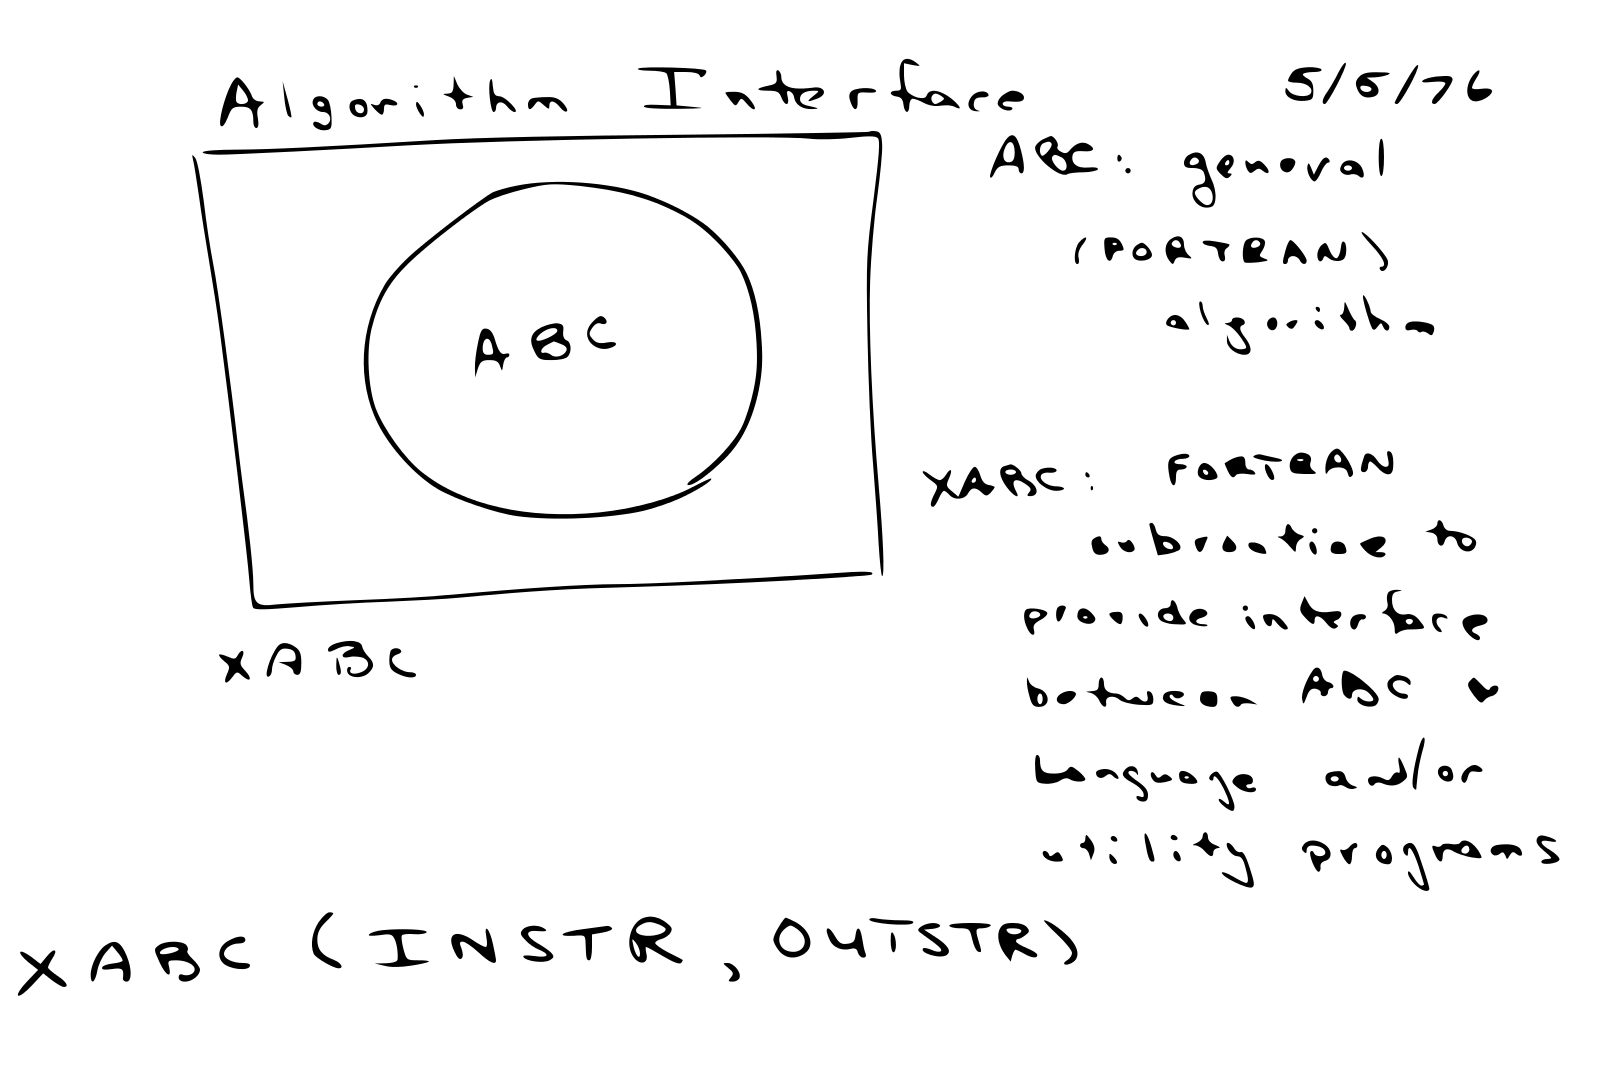
\includegraphics[width=22.22in]{images/01-intro-s-algorithm-interface} \caption{Interface language diagram by John Chambers from useR 2016.}\label{fig:s-diagram}
\end{figure}

R is a modern and free implementation of S, specifically:

\begin{quote}
R is a programming language and free software environment for
statistical computing and graphics.

--- \href{https://www.r-project.org/}{The R Project for Statistical
Computing}
\end{quote}

There are two strong arguments for choosing R over other computing
languages while working with data:

\begin{itemize}
\tightlist
\item
  The \textbf{R Language} was designed by statisticians for
  statisticians, meaning, this is one of the few successful languages
  designed for non-programmers; so learning R will probably feel more
  natural. Additionally, since the R language was designed to be an
  interface to other tools and languages, R allows you to focus more on
  modeling and less on the peculiarities of computer science and
  engineering.
\item
  The \textbf{R Community} provides a rich package archive provided by
  CRAN (\href{https://cran.r-project.org/}{The Comprehensive R Archive
  Network}) which allows you to install ready-to-use packages to perform
  many tasks, most notably, high-quality statistic models with many only
  available in R. In addition, the R community is a welcoming and active
  group of talented individuals motivated to help you succeed. Many
  packages provided by the R community make R, by far, the place to do
  statistical computing.
\end{itemize}

One can argue to what degree other fields, like machine learning,
overlap with statistics; so far, most people will argue that the overlap
is non-trivial. Similar arguments can be made for data science, big
data, deep learning and beyond. With the continuous rise of popularity
of R, I can only expect R's influence and scope to keep growing over
time; we can take a look at the historic downloads of R packages in CRAN
to get some sense of R's recent growth (see Section
\ref{cran-downloads}):

\begin{figure}
\centering
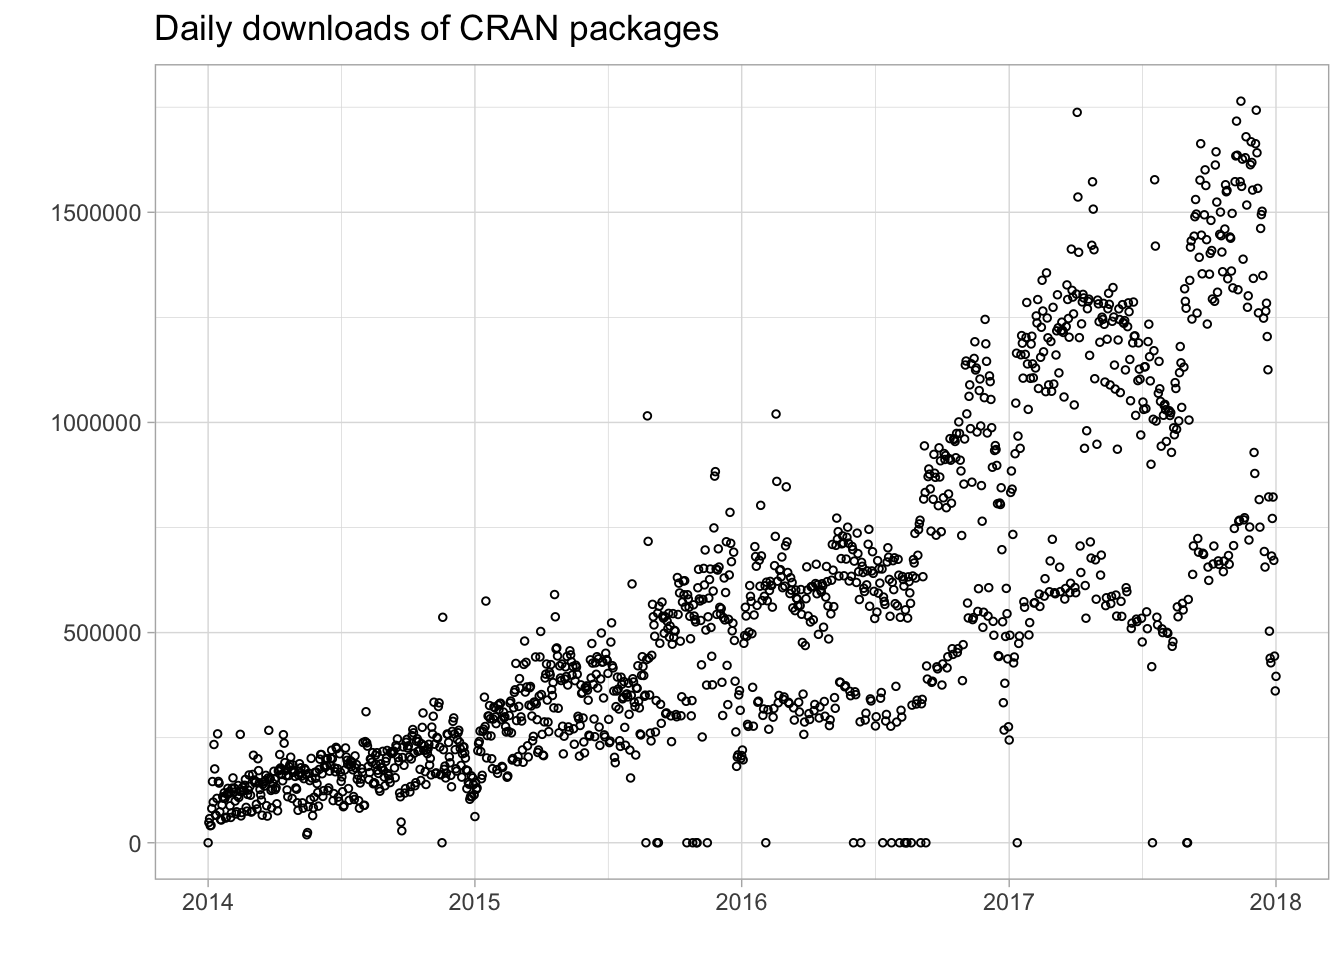
\includegraphics{the-r-in-spark_files/figure-latex/unnamed-chunk-2-1.pdf}
\caption{\label{fig:unnamed-chunk-2}Daily downloads of CRAN packages.}
\end{figure}

\hypertarget{sparklyr}{%
\section{sparklyr}\label{sparklyr}}

Back in 2016, there was a need in the R community to support Spark
through a clean interface compatible with other R packages and available
in CRAN. To this end, development of \texttt{sparklyr} started in 2016
by RStudio under JJ Allaire, Kevin Ushey and Javier Luraschi, version
0.4 was released in summer during the \emph{useR!} conference, this
first version added support for \texttt{dplyr}, \texttt{DBI}, modeling
with \texttt{MLlib} and an extensible API that enabled extensions like
H2Os \href{https://github.com/h2oai/rsparkling/}{rsparkling} package.
Since then, many new features have been added and support across many
Spark distributions and cloud services has made available.

Officially,

\begin{quote}
\texttt{sparklyr} is an R interface for Apache Spark.

---\href{https://github.com/rstudio/sparklyr}{github.com/rstudio/sparklyr}
\end{quote}

It's available in CRAN and works like any other CRAN package, meaning
that: it's agnostic to versions, it's easy to install, it serves the R
community, it embraces other packages and practices from the R community
and so on. It's hosted in GitHub under
\href{github.com/rstudio/sparklyr}{https://github.com/rstudio/sparklyr}
and licensed under Apache 2.0 which is allows you to clone, modify and
contribute back to this project.

While thinking of who and why should use \texttt{sparklyr}, the
following roles come to mind:

\begin{itemize}
\tightlist
\item
  \textbf{New Users}: For new users, I'm going to argue that
  \texttt{sparklyr} is the best way to get started with Spark. My hope
  is that the first chapters of this book will get you up running with
  ease and set you up for long term success.
\item
  \textbf{Data Scientists}: I do believe, strongly, that
  \texttt{sparklyr} in combination with many other R packages and tools
  is the most productive environment for the modern data scientists.
  \texttt{sparklyr} allows support for high-level tasks and low-level
  extensibility mechanisms to match the needs and skills of every data
  scientists.
\item
  \textbf{Expert Users}: For those users that are already immersed in
  Spark and can write code natively inScala, I'm going to argue that
  making their work available as an \texttt{sparklyr} extension is very
  desirable for them and the community. The R community is one of the
  most welcoming and supportive communities I've known, so I can't think
  of better ways of helping the expert users share their work and
  knowledge than by making it available in CRAN to R community.
\end{itemize}

This book is titled ``The R in Spark'' as a way to describe and teach
that area of overlap between Spark and R. The R package that represents
this overlap is \texttt{sparklyr}; however, the overlap goes beyond a
package. It's an overlap of communities, expectations, future
directions, packages and package extensions as well. Naming this book
\texttt{sparklyr} or ``Introduction to sparklyr'' would have left behind
a much more exciting opportunity, an opportunity to present this book as
an intersection of the R and Spark communities. Both are solving very
similar problems with a set of different skills and backgrounds;
therefore, it is my hope that \texttt{sparklyr} can be a fertile ground
for innovation, a welcoming place to newcomers, a productive place for
experienced data scientists and an open community where cluster
computing and modeling can come together.

Here are some resources to help you get involved:

\begin{itemize}
\tightlist
\item
  \textbf{Documentation}: This should be your entry point to learn more
  about sparklyr, the documentation is kept up to date with examples,
  reference functions and many more relevant resources
  (\url{https://spark.rstudio.com}).
\item
  \textbf{Github}: If you believe something needs to get fixed, open a
  GitHub issue or send us a pull request
  (\url{https://github.com/rstudio/sparklyr}).
\item
  \textbf{Stack Overflow}: For general questions, Stack Overflow is a
  good place to start (\url{stackoverflow.com/tags/sparklyr}).
\item
  \textbf{Gitter}: For urgent issues or to keep in touch you can chat
  with us in Gitter (\url{https://gitter.im/rstudio/sparklyr}).
\end{itemize}

\hypertarget{started}{%
\chapter{Getting Started}\label{started}}

From R, installing and launching a local Spark cluster using
\texttt{sparklyr} is as easy as running:

\begin{Shaded}
\begin{Highlighting}[]
\KeywordTok{spark_install}\NormalTok{()}
\NormalTok{sc <-}\StringTok{ }\KeywordTok{spark_connect}\NormalTok{(}\DataTypeTok{master =} \StringTok{"local"}\NormalTok{)}
\end{Highlighting}
\end{Shaded}

However, to make sure we can all run the code above and understand it,
this section will walk you through installing the prerequisites,
installing Spark and connecting to a local Spark cluster.

\hypertarget{prerequisites}{%
\section{Prerequisites}\label{prerequisites}}

As briefly mentioned in Section \ref{intro}, R is a programming language
that can run in many platforms and environments. Most people making use
of a programming language also choose tools to make them more productive
in it; for R, RStudio would be such tool. Strictly speaking, RStudio is
an Integrated Development Environment or IDE for short, which also
happens to support many platforms and environments. R and RStudio are
the free software tools this book will make use of and therefore, I
strongly recommend you get those installed if you haven't done so
already.

Additionally, since Spark is build in the Scala programming language
which is run by the Java Virtual Machine, you also need to install Java
7 or newer in your system. It is likely that your system already has
Java installed, but is probably worth updating with the steps bellow.

\hypertarget{install-r}{%
\subsection{Install R}\label{install-r}}

From \href{https://r-project.org/}{r-project.org}, download and launch
the installer for your platform, Windows, Macs or Linux available.

\begin{figure}

{\centering 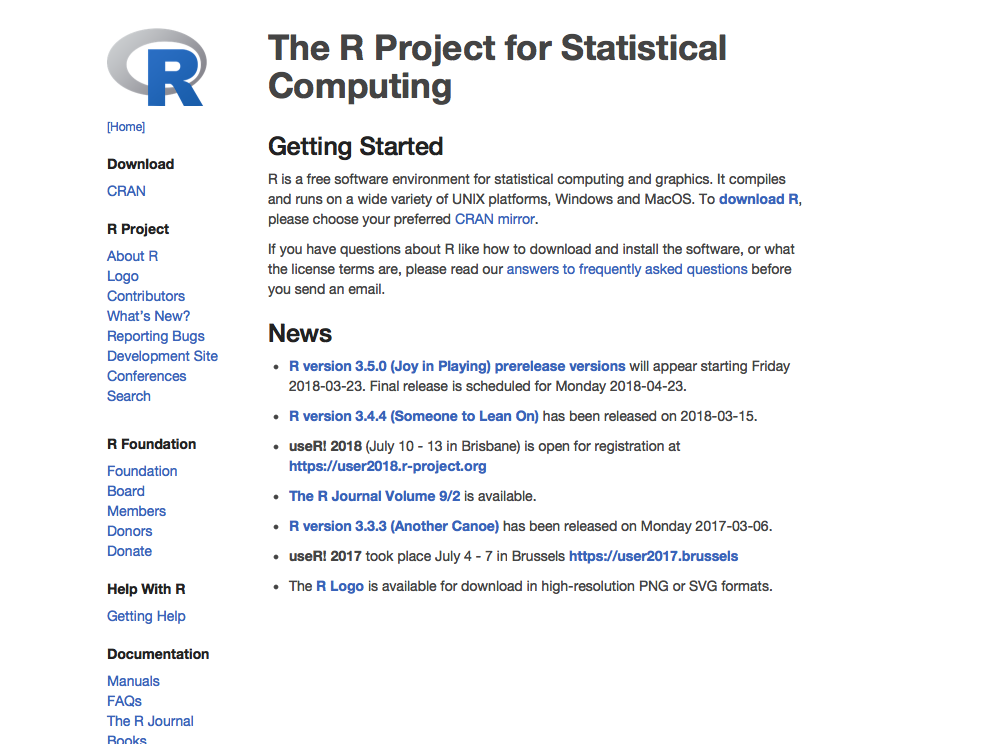
\includegraphics{the-r-in-spark_files/figure-latex/r-download-1} 

}

\caption{The R Project for Statistical Computing.}\label{fig:r-download}
\end{figure}

\hypertarget{install-java}{%
\subsection{Install Java}\label{install-java}}

From
\href{http://www.oracle.com/technetwork/java/javase/downloads/jdk8-downloads-2133151.html}{oracle.com/technetwork/java/javase/downloads/jdk8-downloads-2133151.html},
download and launch the installer for your platform, Windows, Macs or
Linux available. While installing the JRE (Java Runtime Environment) is
sufficient for most operations, in order to build extensions you will
need the JDK (Java Developer Kit); therefore, I rather recommend
installing the JDK in the first place.

\begin{figure}

{\centering 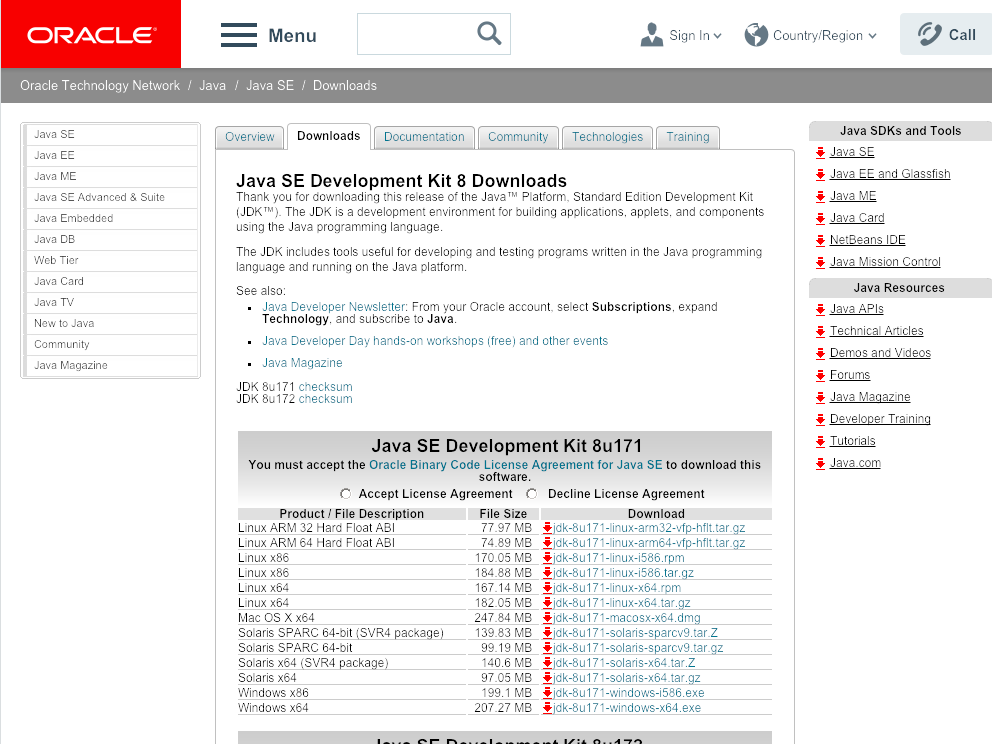
\includegraphics[width=13.78in]{images/02-getting-started-jdk-8} 

}

\caption{Java Download.}\label{fig:java-download}
\end{figure}

\hypertarget{install-rstudio}{%
\subsection{Install RStudio}\label{install-rstudio}}

While installing RStudio is not strictly required to work with
\texttt{sparklyr} in R, it will make you much more production and
therefore, I highly recommend you take the time to install RStudio from
\href{https://www.rstudio.com/products/rstudio/download/}{rstudio.com/products/rstudio/download/},
then download and launch the installer for your platform, Windows, Macs
or Linux available.

\begin{figure}

{\centering 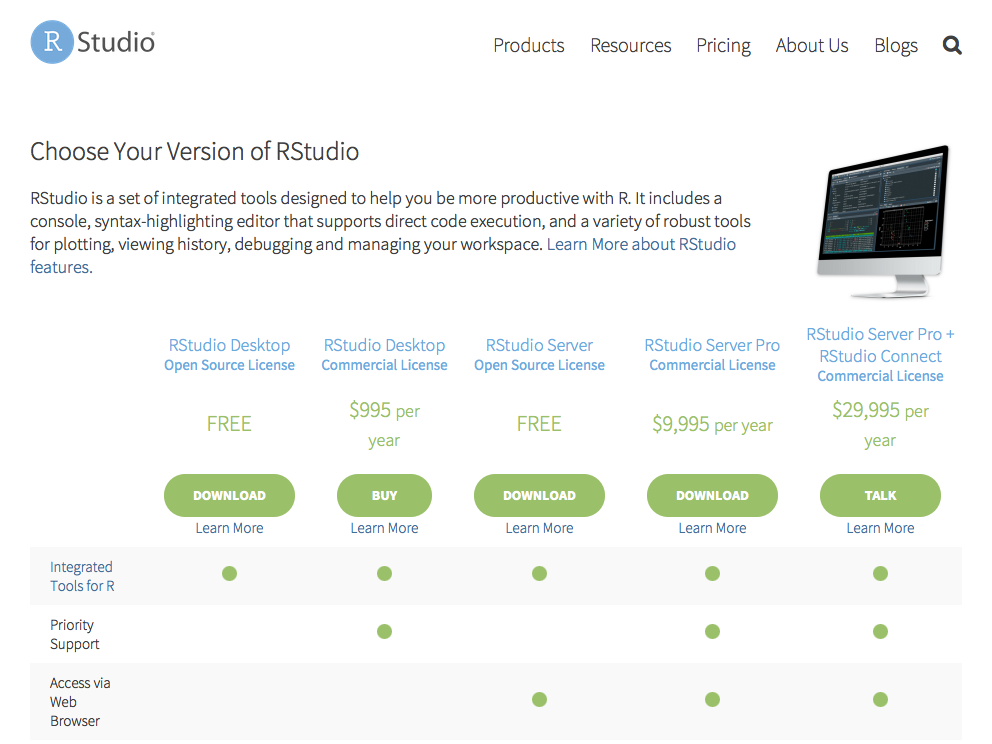
\includegraphics[width=13.78in]{images/02-getting-started-rstudio} 

}

\caption{RStudio Downloads.}\label{fig:rstudio-download}
\end{figure}

After launching RStudio, identify the Console panel since this is where
most of the code will be executed in this book. For additional learning
resources on R and RStudio consider visiting:
\href{https://www.rstudio.com/online-learning/}{rstudio.com/online-learning/}.

\hypertarget{install-sparklyr}{%
\subsection{Install sparklyr}\label{install-sparklyr}}

First of all, we would want to install \texttt{sparkylr}. As many other
R packages, \texttt{sparklyr} is available in
\href{https://CRAN.R-project.org/package=sparklyr}{CRAN} and can be
easily installed as follows:

\begin{Shaded}
\begin{Highlighting}[]
\KeywordTok{install.packages}\NormalTok{(}\StringTok{"sparklyr"}\NormalTok{)}
\end{Highlighting}
\end{Shaded}

The CRAN release of \texttt{sparklyr} contains the most stable version
and it's the recommended version to use; however, for those that need or
might want to try newer features being developed in \texttt{sparklyr}
you can install directly from GitHub using the \texttt{devtools}
package. First install the \texttt{devtools} package and then
\texttt{sparklyr} as follows:

\begin{Shaded}
\begin{Highlighting}[]
\KeywordTok{install.packages}\NormalTok{(}\StringTok{"devtools"}\NormalTok{)}
\NormalTok{devtools}\OperatorTok{::}\KeywordTok{install_github}\NormalTok{(}\StringTok{"rstudio/sparklyr"}\NormalTok{)}
\end{Highlighting}
\end{Shaded}

\hypertarget{installing-spark}{%
\section{Installing Spark}\label{installing-spark}}

Start by loading \texttt{sparklyr},

\begin{Shaded}
\begin{Highlighting}[]
\KeywordTok{library}\NormalTok{(sparklyr)}
\end{Highlighting}
\end{Shaded}

This will makes all \texttt{sparklyr} functions available in R, which is
really helpful; otherwise, we would have to run each \texttt{sparklyr}
command prefixed with \texttt{sparklyr::}.

As mentioned, Spark can be easily installed by running
\texttt{spark\_install()}; this will install the latest version of Spark
locally in your computer, go ahead and run \texttt{spark\_install()}.
Notice that this command requires internet connectivity to download
Spark.

\begin{Shaded}
\begin{Highlighting}[]
\KeywordTok{spark_install}\NormalTok{()}
\end{Highlighting}
\end{Shaded}

All the versions of Spark that are available for installation can be
displayed with \texttt{spark\_available\_versions()}:

\begin{Shaded}
\begin{Highlighting}[]
\KeywordTok{spark_available_versions}\NormalTok{()}
\end{Highlighting}
\end{Shaded}

\begin{verbatim}
##    spark
## 1  1.6.3
## 2  1.6.2
## 3  1.6.1
## 4  1.6.0
## 5  2.0.0
## 6  2.0.1
## 7  2.0.2
## 8  2.1.0
## 9  2.1.1
## 10 2.2.0
## 11 2.2.1
## 12 2.3.0
\end{verbatim}

A specific version can be installed using the Spark version and,
optionally, by also specifying the Hadoop version. For instance, to
install Spark 1.6.3, we would run \texttt{spark\_install("1.6.3")}.

You can also check which versions are installed by running:

\begin{Shaded}
\begin{Highlighting}[]
\KeywordTok{spark_installed_versions}\NormalTok{()}
\end{Highlighting}
\end{Shaded}

Finally, in order to uninstall an specific version of Spark you can run
\texttt{spark\_uninstall()} by specifying the Spark and Hadoop versions,
for instance:

\begin{Shaded}
\begin{Highlighting}[]
\KeywordTok{spark_uninstall}\NormalTok{(}\DataTypeTok{version =} \StringTok{"1.6.0"}\NormalTok{, }\DataTypeTok{hadoop =} \StringTok{"2.6"}\NormalTok{)}
\end{Highlighting}
\end{Shaded}

\hypertarget{connecting-to-spark}{%
\section{Connecting to Spark}\label{connecting-to-spark}}

It's important to mention that, so far, we've only installed a local
Spark cluster. A local cluster is really helpful to get started, test
code and troubleshoot with ease; further chapters will explain where to
find, install and connect to real Spark clusters with many machines; but
for the first few chapters, we will focus on using local clusters.

Threfore, to connect to this local cluster we simple run:

\begin{Shaded}
\begin{Highlighting}[]
\NormalTok{sc <-}\StringTok{ }\KeywordTok{spark_connect}\NormalTok{(}\DataTypeTok{master =} \StringTok{"local"}\NormalTok{)}
\end{Highlighting}
\end{Shaded}

The \texttt{master} parameter helps \texttt{sparklyr} find which is the
``main'' machine from the Spark cluster, this machine is often call the
driver node. While working with real clusters using many machines, most
machines will be worker machines and one will be the master. Since we
only have a local cluster with only one machine, we will default to use
\texttt{"local"} for now.

\hypertarget{using-spark}{%
\section{Using Spark}\label{using-spark}}

Now that you are connected, we can run a simple commands. For instance,
let's start by loading some text.

First, lets create a text file by running:

\begin{Shaded}
\begin{Highlighting}[]
\KeywordTok{write}\NormalTok{(}\StringTok{"Hello World!"}\NormalTok{, }\StringTok{"hello.txt"}\NormalTok{)}
\end{Highlighting}
\end{Shaded}

Which we can read back in Spark by running:

\begin{Shaded}
\begin{Highlighting}[]
\KeywordTok{spark_read_text}\NormalTok{(sc, }\StringTok{"hello"}\NormalTok{, }\StringTok{"hello.txt"}\NormalTok{)}
\end{Highlighting}
\end{Shaded}

\begin{verbatim}
## # Source:   table<hello> [?? x 1]
## # Database: spark_connection
##   line        
##   <chr>       
## 1 Hello World!
\end{verbatim}

\hypertarget{web-interface}{%
\subsection{Web Interface}\label{web-interface}}

Most of the Spark commands will get started from the R console; however,
it is often the case that monitoring and analizing execution is done
through Spark's web interface. This interface is a web page provided by
the driver node which can be accessed from \texttt{sparklyr} by running:

\begin{Shaded}
\begin{Highlighting}[]
\KeywordTok{spark_web}\NormalTok{(sc)}
\end{Highlighting}
\end{Shaded}

\begin{figure}

{\centering 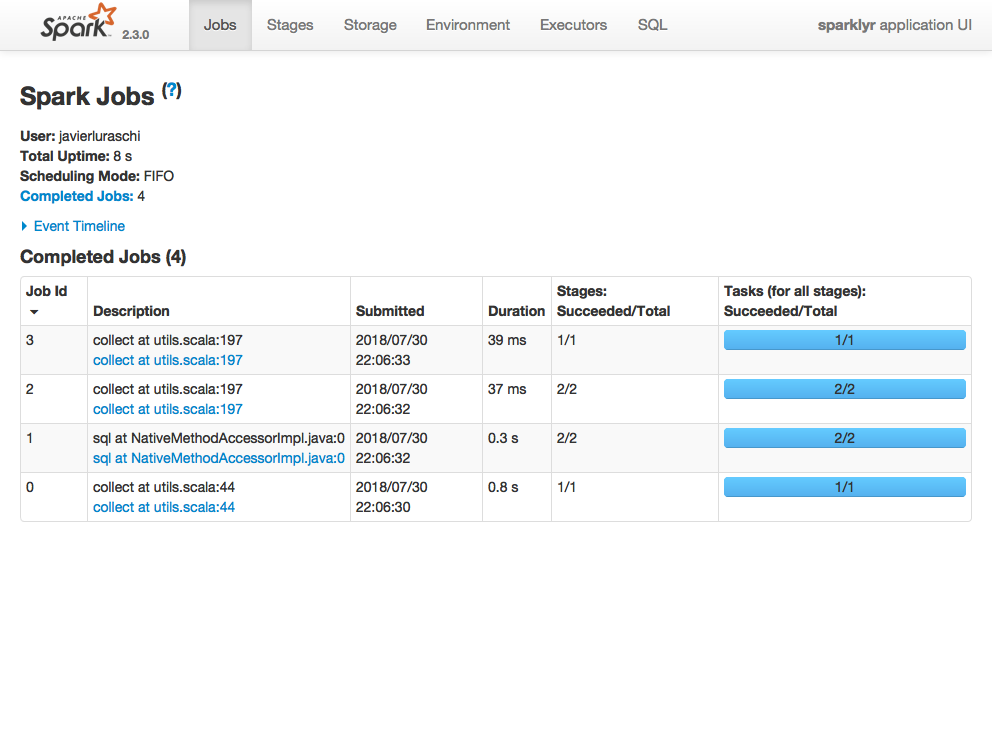
\includegraphics[width=13.78in]{images/02-getting-started-spark-web} 

}

\caption{Apache Spark Web Interface.}\label{fig:spark-web}
\end{figure}

\hypertarget{logs}{%
\subsection{Logs}\label{logs}}

Another common tool is to read through the Spark logs, a log is just a
text file where Spark will append information relevant to the execution
of tasks in the cluster. For local clusters, we can retrieve the
\texttt{sparklyr} related log entries by running:

\begin{Shaded}
\begin{Highlighting}[]
\KeywordTok{spark_log}\NormalTok{(sc, }\DataTypeTok{filter =} \StringTok{"sparklyr"}\NormalTok{, }\DataTypeTok{n =} \DecValTok{5}\NormalTok{)}
\end{Highlighting}
\end{Shaded}

\begin{verbatim}
## 18/04/19 22:25:03 INFO SparkContext: Submitted application: sparklyr
## 18/04/19 22:25:04 INFO SparkContext: Added JAR file:/Library/Frameworks/R.framework/Versions/3.4/Resources/library/sparklyr/java/sparklyr-2.2-2.11.jar at spark://127.0.0.1:55445/jars/sparklyr-2.2-2.11.jar with timestamp 1524201904194
## 18/04/19 22:25:10 INFO Executor: Fetching spark://127.0.0.1:55445/jars/sparklyr-2.2-2.11.jar with timestamp 1524201904194
## 18/04/19 22:25:10 INFO Utils: Fetching spark://127.0.0.1:55445/jars/sparklyr-2.2-2.11.jar to /private/var/folders/fz/v6wfsg2x1fb1rw4f6r0x4jwm0000gn/T/spark-bc2b9a07-421c-4130-8d4d-59a98d9f9b9a/userFiles-4e80b486-36e0-480b-abf1-e2ac62e7a11a/fetchFileTemp7505929974481292946.tmp
## 18/04/19 22:25:10 INFO Executor: Adding file:/private/var/folders/fz/v6wfsg2x1fb1rw4f6r0x4jwm0000gn/T/spark-bc2b9a07-421c-4130-8d4d-59a98d9f9b9a/userFiles-4e80b486-36e0-480b-abf1-e2ac62e7a11a/sparklyr-2.2-2.11.jar to class loader
\end{verbatim}

\hypertarget{disconnecting}{%
\section{Disconnecting}\label{disconnecting}}

For local clusters and, really, any cluster; once you are done
processing data you should disconnect by running:

\begin{Shaded}
\begin{Highlighting}[]
\KeywordTok{spark_disconnect}\NormalTok{(sc)}
\end{Highlighting}
\end{Shaded}

this will terminate the connection to the cluster but also terminate the
cluster tasks as well. If multiple Spark connections are active, or if
the conneciton instance \texttt{sc} is no longer available, you can also
disconnect all your Spark connections by running
\texttt{spark\_disconnect\_all()}.

\hypertarget{recap}{%
\section{Recap}\label{recap}}

This chapter walked you through installing R, Java, RStudio and
\texttt{sparklyr} as the main tools required to use Spark from R. We
covered installing local Spark clusters using \texttt{spark\_install()}
and learned how to launch the web interface using
\texttt{spark\_web(sc)} and view logs using \texttt{spark\_log(sc)}.

It is my hope that this chapter will help anyone interested in learning
cluster computing using Spark and R to get you started, ready to
experiment on your own and ready to tackle actual data analysis and
modeling tasks without any makor blockers. However, if you hit any
installation or connection issues, start by browsing online for the
error message or open a GitHub issue under
\url{https://github.com/rstudio/sparklyr/issues} to help you get going.

\hypertarget{dplyr}{%
\chapter{Data Analysis}\label{dplyr}}

\hypertarget{dplyr-1}{%
\section{dplyr}\label{dplyr-1}}

\hypertarget{dbi}{%
\section{DBI}\label{dbi}}

\hypertarget{modeling}{%
\chapter{Modeling}\label{modeling}}

\hypertarget{mllib}{%
\section{mllib}\label{mllib}}

\hypertarget{clusters}{%
\chapter{Clusters}\label{clusters}}

Previous chapters focused on using Spark over a single computing
instance, your personal computer. In this chapter we will introduce
techniques to run Spark over multiple computing instances to do proper
data science at scale.

However, you might already have a Spark cluster in your organization,
being that the case, you could consider skipping to the next chapter,
Connections, which will teach you how to connect to an existing
clusters.

For those that don't have a cluster or are considering improvements to
their existing infrastructure, this chapter will introduce the most
common cluster architectures available today.

\hypertarget{overview}{%
\section{Overview}\label{overview}}

While working with clusters of many computing instances, you will need
to find enough computing instances to perform de computation at the
scale you intend. There are two options available today known as
\emph{on-prem} or \emph{cloud}.

\emph{On-prem} stands for on-premise, meaning that someone, either
yourself or someone in your organiation purchased physical computers
that are intended to be used for cluster computing. The computers in
this cluster can made of \emph{off-the-shelf} hardware, meaning that
someone place an order to purchase computers usually found in stores
shelves or, \emph{high-performance} hardware, meaning that a computing
vendor provided highly customized computing hardware which also comes
optimized for high-performance network connectivity, power consumption,
etc. When purchasing hundreds or thousands of computing instances, it
doesn't make sense to keep them in the usual computing casing that we
are all familiar with, but rather, it makes sense to stack them as
efficient as possible on top of each other to minimize space and help
disipate heat. This group of efficiently stacked computing instances is
known as a \href{https://en.wikipedia.org/wiki/Rack_unit}{rack}. Once
you have thousands or, yes, even millions of computers, you will also
need many racks of computing devices and yes, you would also need
significant physycal space to hosts those racks, a building that
provides racks of computing instances is usually known as a Data Center.
A data center is a building designated to hold many racks with many
computing instances in each. At the scale of a data center, optimizing
the building that holds them, their heating system, power suply, network
connectivity, etc. becomes also relevant to optimize. In 2011, Facebook
\href{https://code.facebook.com/posts/187637061409082/building-efficient-data-centers-with-the-open-compute-project/}{announced}
the \href{http://www.opencompute.org/}{Open Compute Project} inniciative
which provides a set of data center blueprints free for anyone to use.

There is nothing preventing us from building our own data centers and in
fact, many organizations have followed this path. For instance, Amazon
started as an online book store, over the years Amazon grew to sell much
more than just books and, with it's online store growth, their data
centers also grew in size. In 2002, Amazon considered
\href{https://en.wikipedia.org/wiki/Amazon_Web_Services\#History}{selling
access to virtual servers}, in their data centers to the public and, in
2004, Amazon Web Services launched as a way to let anyone rent a subset
of their datacenters on-demand, meaning that one did not have to
purchase, configure, maintain nor teardown it's own clusters but could
rather rent them from Amazon directly. cloud computing.

The on-demand compute model is what we know today as \emph{Cloud} and
stands for Cloud Computing. It's a concept that evolved from Amazon Web
Services providing their data centers as a service. In the cloud, the
cluster you use is not owned by you and is neither in your physical
building, but rather, it's a data center owned and managed by someone
else. Today, there are many cloud providers in this space ranging from
Amazon, Microsoft, Google, IBM and many others. Most cloud computing
platforms provide a user interface either through a web applciation and
command line to request resources, connect to them and tear them down

\begin{figure}
\centering
\includegraphics{the-r-in-spark_files/figure-latex/unnamed-chunk-17-1.pdf}
\caption{\label{fig:unnamed-chunk-17}Google trends for mainframes, cloud
computing and kubernetes.}
\end{figure}

\hypertarget{on-prem-vs-cloud}{%
\section{On-Prem vs Cloud}\label{on-prem-vs-cloud}}

First, we can start by asking where are the machines for your cluster
will be located? For historical reasons, most organizations have choosen
to colocate their cluster machiens with their business, as in, there is
a room full of computers hosting a variety of software. More recently,
software companies have made available clusters of machines available in
their own data centers that one can connect to and rent. We call the
former, on-premise cluster or on-prem for short and, cloud clusters or
on-demand cluster for the latter one. Each have different tradeoffs
worth considering.

For those readers that already have an Spark cluster in their
organization, you should ask your cluster administrator to provide
connection information for this cluster and read carefully their usage
policies and constraints. A cluster is usually shared among many users
so you want to be respectful of others time and resources while using a
shared cluster environment. Your system administrator will describe if
it's an \textbf{on-prem} vs \textbf{cloud} cluster, the
\textbf{distribution}, the cluster \textbf{manager} being used,
supported \textbf{connections} and supported \textbf{tools}.

For those readers that don't have a cluster yet, it is likely that you
will want to choose a cloud cluster, reading throught this chapter will
help you an overview of all the different approaches you can take to
create your own cluster or decide which cluster provider to use. At the
end, there is no right answer for all readers, but my hope if that this
will help you take a sensible decision on which cluster provider and
distribution to choose.

\hypertarget{on-prem}{%
\subsection{On-Prem}\label{on-prem}}

For on-premise clusters, a set of machines is managed by an
organization. The machines are usually colocated with their physical
location and are managed by staff usually employed by their
organization. These clusters can be highly customized and controlled;
however, they inccur significant initial expenses and high management
costs.

\textbf{Cloudera}

\begin{figure}

{\centering 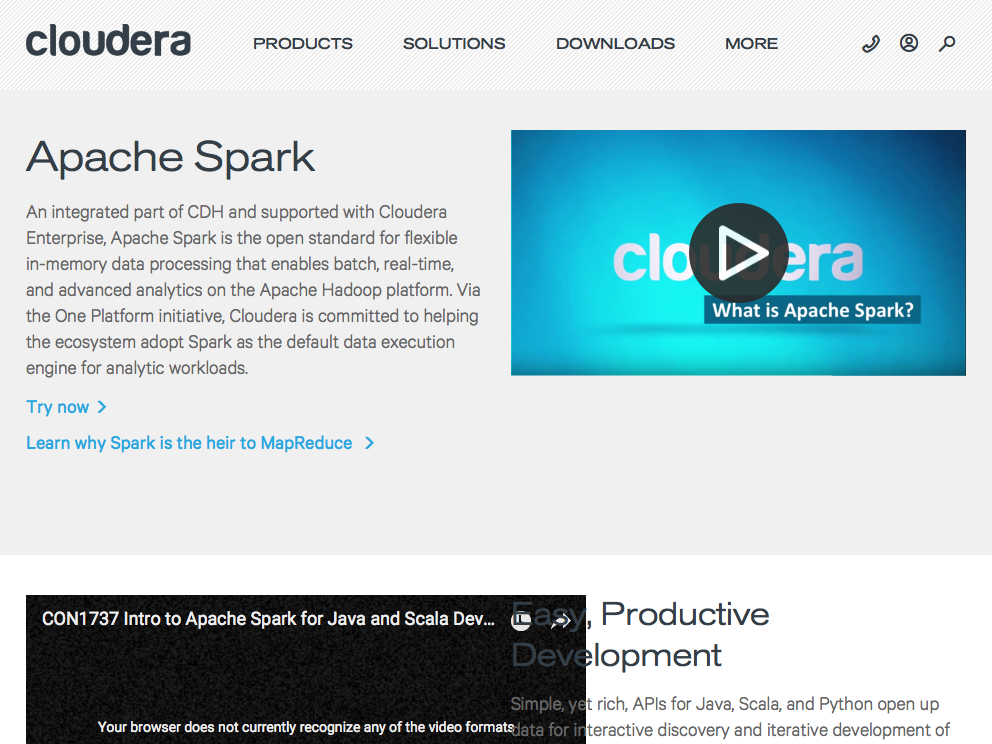
\includegraphics[width=13.78in]{images/05-clusters-cloudera-landing} 

}

\caption{Cloudera Landing Site.}\label{fig:cloudera-spark}
\end{figure}

\textbf{Hortonworks}

\begin{figure}

{\centering 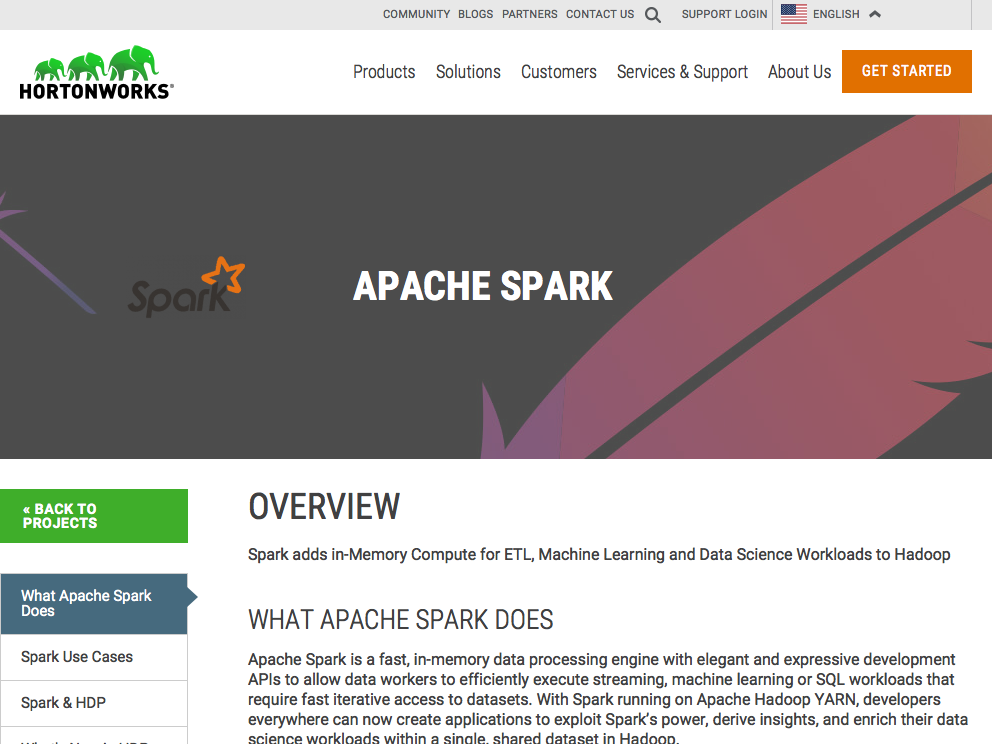
\includegraphics[width=13.78in]{images/05-clusters-hortonworks-landing} 

}

\caption{Hortonworks Landing Site.}\label{fig:hortonworks-spark}
\end{figure}

\textbf{MapR}

\begin{figure}

{\centering 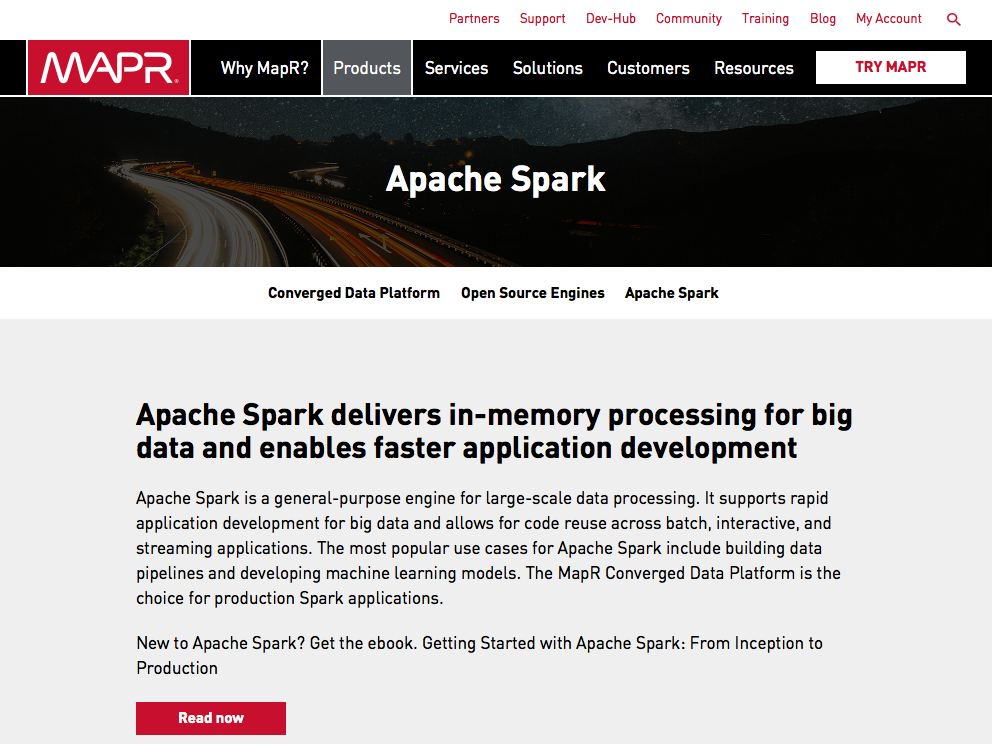
\includegraphics[width=13.78in]{images/05-clusters-mapr-landing} 

}

\caption{MapR Landing Site.}\label{fig:mapr-spark}
\end{figure}

\hypertarget{cloud}{%
\subsection{Cloud}\label{cloud}}

For cloud clusters, the machines are rented from a cloud provider by an
hourly and even by the minute or second basis. The cloud providers with
highest market captical are: Amazon, Google and Microsoft.

\textbf{Amazon} provides cloud services through
\href{https://aws.amazon.com/}{Amazon Web Services}; more specifically,
they provide an on-demand Spark cluster through
\href{https://aws.amazon.com/emr/}{Amazon Elastic Mad Reduce} or EMR for
short.

\begin{figure}

{\centering 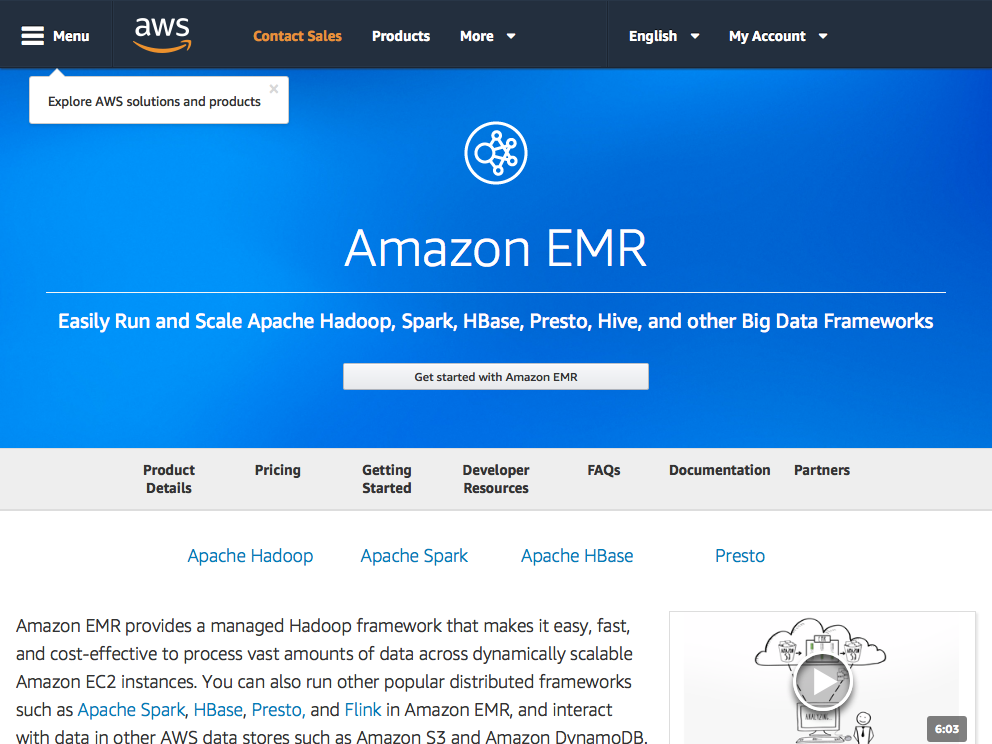
\includegraphics[width=13.78in]{images/05-clusters-amazon-emr-landing} 

}

\caption{Amazon EMR Landing Site.}\label{fig:amazon-emr}
\end{figure}

\textbf{Google} provides their on-demand computing services through
their \href{https://cloud.google.com/}{Google Cloud}, on-demand Spark
cluster are provided by \href{https://cloud.google.com/dataproc/}{Google
Dataproc}.

\begin{figure}

{\centering 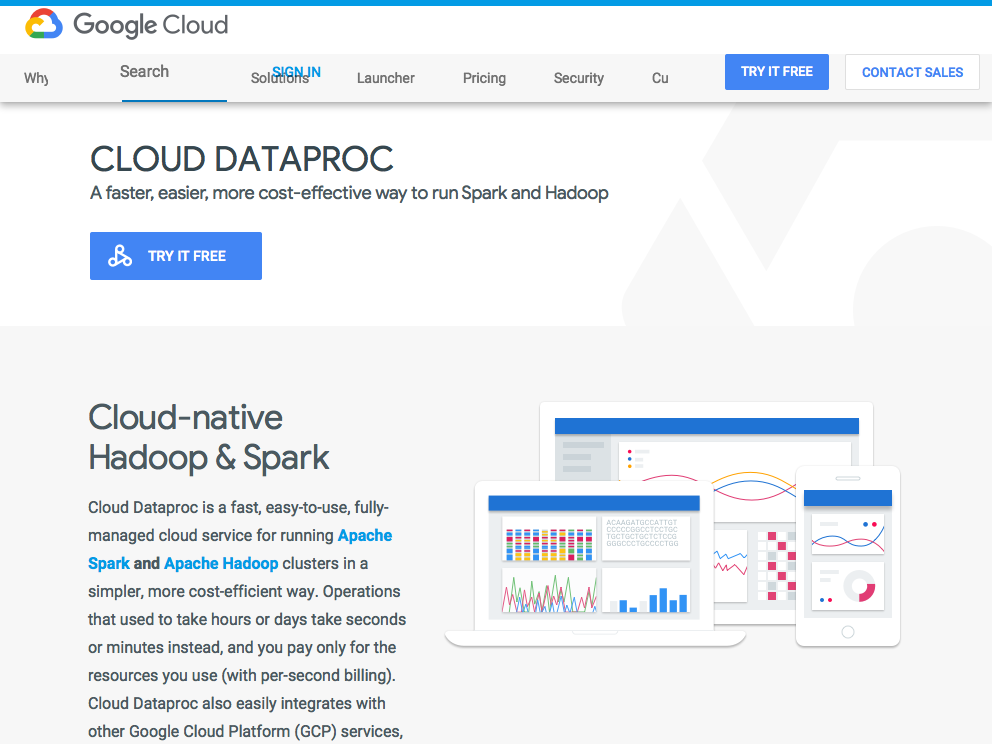
\includegraphics[width=13.78in]{images/05-clusters-dataproc-landing} 

}

\caption{Google Dataprox Landing Site.}\label{fig:google-dataproc}
\end{figure}

\textbf{Microsoft} provides cloud services thorugh
\href{https://azure.microsoft.com/}{Microsft Azure} and Spark clusters
through
\href{https://azure.microsoft.com/en-us/services/hdinsight/}{Azure
HDInsight}.

\begin{figure}

{\centering 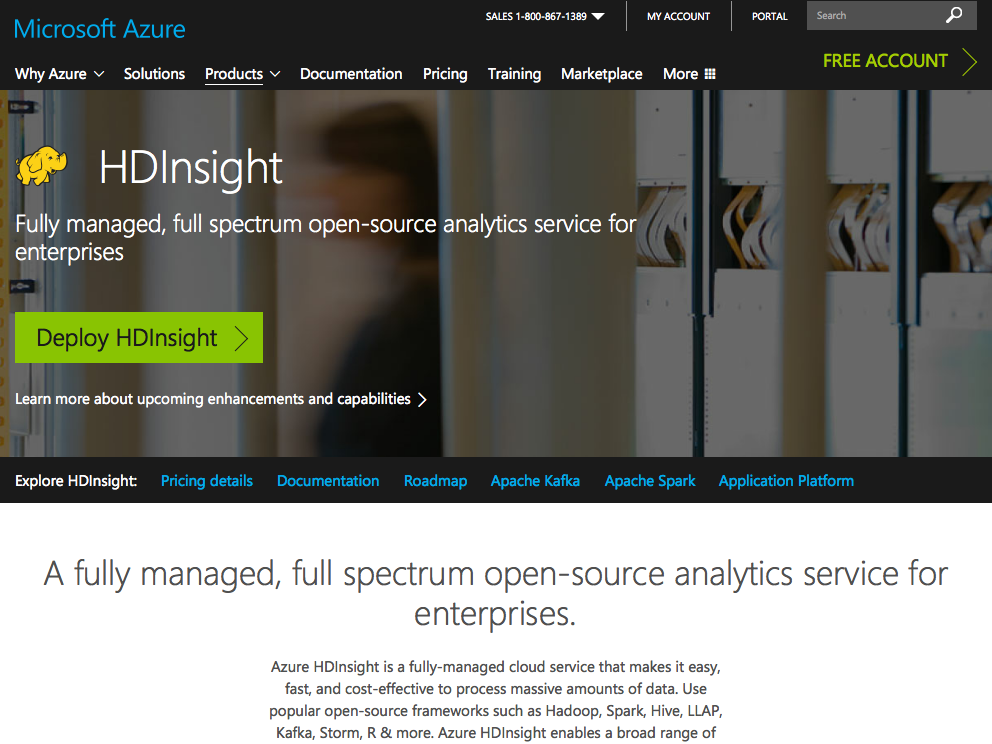
\includegraphics[width=13.78in]{images/05-clusters-azure-landing} 

}

\caption{Azure HDInsight Landing Site.}\label{fig:azure-hdinsight}
\end{figure}

\hypertarget{distributions}{%
\section{Distributions}\label{distributions}}

\hypertarget{managers}{%
\section{Managers}\label{managers}}

While running Spark over multiple machines, the first challenge one
would encounter is how to manage all those machines with ease. One
approach would be to manually set up and configure Spark over each
machine, while possible, this is usually impractical due to the
innificiencies of managing one machine at a time; instead of installing
Spark, Hadoop, etc. manually over every machine, what is known as a
\href{https://en.wikipedia.org/wiki/Cluster_manager}{cluster manager} is
usually installed only once. Once a cluster manager is installed, it
will provide the tools to install additional software over each node,
Hadoop, Spark, etc. There are many cluster managers

\hypertarget{standalone}{%
\subsection{Standalone}\label{standalone}}

\hypertarget{yarn}{%
\subsection{Yarn}\label{yarn}}

\hypertarget{mesos}{%
\subsection{Mesos}\label{mesos}}

\hypertarget{kubernetes}{%
\subsection{Kubernetes}\label{kubernetes}}

\hypertarget{livy}{%
\subsection{Livy}\label{livy}}

\begin{figure}

{\centering 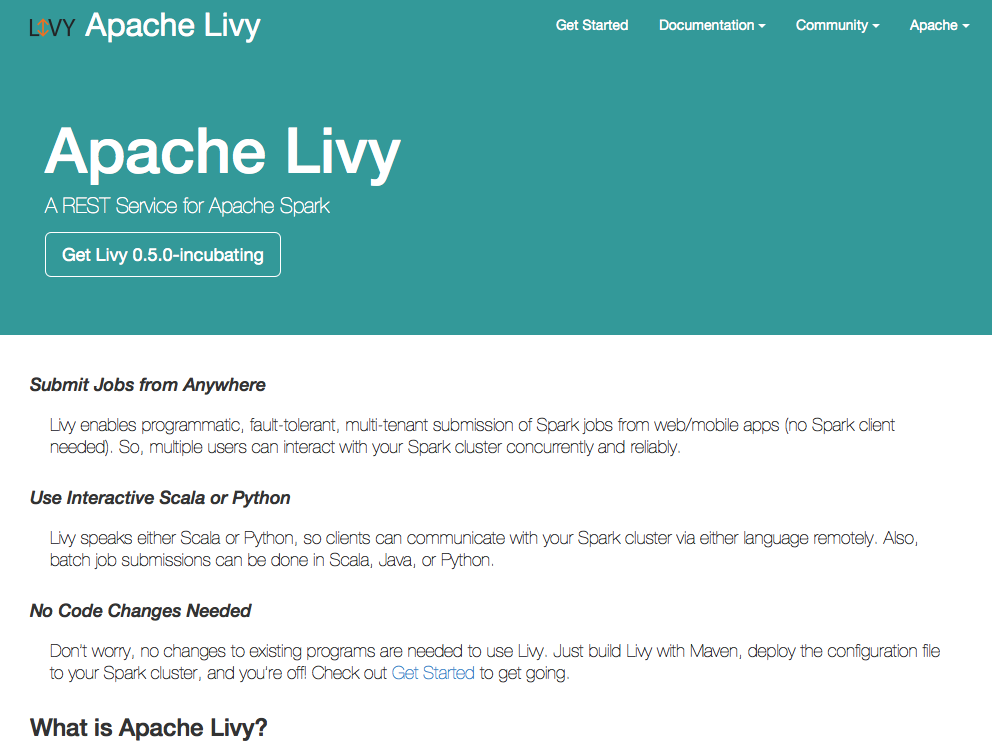
\includegraphics[width=13.78in]{images/05-clusters-apache-livy} 

}

\caption{Apache Livy.}\label{fig:apache-livy}
\end{figure}

\hypertarget{remote-clusters}{%
\section{Remote Clusters}\label{remote-clusters}}

In this section we will explore how to connect

\hypertarget{same-network}{%
\subsection{Same Network}\label{same-network}}

\hypertarget{different-network}{%
\subsection{Different Network}\label{different-network}}

Connecting from RStudio Server to remote Spark

\hypertarget{connections}{%
\chapter{Connections}\label{connections}}

\hypertarget{overview-1}{%
\section{Overview}\label{overview-1}}

\hypertarget{local}{%
\section{Local}\label{local}}

\hypertarget{spark-1}{%
\section{Spark}\label{spark-1}}

\hypertarget{yarn-1}{%
\section{Yarn}\label{yarn-1}}

\hypertarget{client}{%
\subsection{Client}\label{client}}

\hypertarget{server}{%
\subsection{Server}\label{server}}

\hypertarget{mesos-1}{%
\section{Mesos}\label{mesos-1}}

\hypertarget{livy-1}{%
\section{Livy}\label{livy-1}}

\hypertarget{data}{%
\chapter{Data Sources}\label{data}}

\hypertarget{csv}{%
\section{CSV}\label{csv}}

\hypertarget{text}{%
\section{Text}\label{text}}

\hypertarget{parquet}{%
\section{Parquet}\label{parquet}}

\hypertarget{jdbc}{%
\section{JDBC}\label{jdbc}}

\hypertarget{others}{%
\section{Others}\label{others}}

\hypertarget{tuning}{%
\chapter{Tuning}\label{tuning}}

\hypertarget{caching}{%
\section{Caching}\label{caching}}

\hypertarget{partitions}{%
\section{Partitions}\label{partitions}}

\hypertarget{shuffling}{%
\section{Shuffling}\label{shuffling}}

\hypertarget{checkpointing}{%
\section{Checkpointing}\label{checkpointing}}

\hypertarget{extensions}{%
\chapter{Extensions}\label{extensions}}

\hypertarget{using-extensions}{%
\section{Using Extensions}\label{using-extensions}}

\hypertarget{writting-extensions}{%
\section{Writting Extensions}\label{writting-extensions}}

\hypertarget{distributed}{%
\chapter{Distributed R}\label{distributed}}

\hypertarget{use-cases}{%
\section{Use Cases}\label{use-cases}}

\hypertarget{troubleshooting}{%
\section{Troubleshooting}\label{troubleshooting}}

\hypertarget{appendix}{%
\chapter*{Appendix}\label{appendix}}
\addcontentsline{toc}{chapter}{Appendix}

\hypertarget{storage-capacity}{%
\section{Worlds Store Capacity}\label{storage-capacity}}

\begin{Shaded}
\begin{Highlighting}[]
\KeywordTok{library}\NormalTok{(tidyverse)}
\KeywordTok{read_csv}\NormalTok{(}\StringTok{"data/01-worlds-capacity-to-store-information.csv"}\NormalTok{, }\DataTypeTok{skip =} \DecValTok{8}\NormalTok{) }\OperatorTok
\StringTok{  }\KeywordTok{gather}\NormalTok{(}\DataTypeTok{key =}\NormalTok{ storage, }\DataTypeTok{value =}\NormalTok{ capacity, analog, digital) }\OperatorTok
\StringTok{  }\KeywordTok{mutate}\NormalTok{(}\DataTypeTok{year =}\NormalTok{ X1, }\DataTypeTok{terabytes =}\NormalTok{ capacity }\OperatorTok{/}\StringTok{ }\FloatTok{1e+12}\NormalTok{) }\OperatorTok
\StringTok{  }\KeywordTok{ggplot}\NormalTok{(}\KeywordTok{aes}\NormalTok{(}\DataTypeTok{x =}\NormalTok{ year, }\DataTypeTok{y =}\NormalTok{ terabytes, }\DataTypeTok{group =}\NormalTok{ storage)) }\OperatorTok{+}
\StringTok{    }\KeywordTok{geom_line}\NormalTok{(}\KeywordTok{aes}\NormalTok{(}\DataTypeTok{linetype =}\NormalTok{ storage)) }\OperatorTok{+}
\StringTok{    }\KeywordTok{geom_point}\NormalTok{(}\KeywordTok{aes}\NormalTok{(}\DataTypeTok{shape =}\NormalTok{ storage)) }\OperatorTok{+}
\StringTok{    }\KeywordTok{scale_y_log10}\NormalTok{(}
      \DataTypeTok{breaks =}\NormalTok{ scales}\OperatorTok{::}\KeywordTok{trans_breaks}\NormalTok{(}\StringTok{"log10"}\NormalTok{, }\ControlFlowTok{function}\NormalTok{(x) }\DecValTok{10}\OperatorTok{^}\NormalTok{x),}
      \DataTypeTok{labels =}\NormalTok{ scales}\OperatorTok{::}\KeywordTok{trans_format}\NormalTok{(}\StringTok{"log10"}\NormalTok{, scales}\OperatorTok{::}\KeywordTok{math_format}\NormalTok{(}\DecValTok{10}\OperatorTok{^}\NormalTok{x))}
\NormalTok{    ) }\OperatorTok{+}
\StringTok{    }\KeywordTok{theme_light}\NormalTok{() }\OperatorTok{+}
\StringTok{    }\KeywordTok{theme}\NormalTok{(}\DataTypeTok{legend.position =} \StringTok{"bottom"}\NormalTok{)}
\end{Highlighting}
\end{Shaded}

\hypertarget{cran-downloads}{%
\section{Daily downloads of CRAN packages}\label{cran-downloads}}

\begin{Shaded}
\begin{Highlighting}[]
\NormalTok{downloads_csv <-}\StringTok{ "data/01-intro-r-cran-downloads.csv"}
\ControlFlowTok{if}\NormalTok{ (}\OperatorTok{!}\KeywordTok{file.exists}\NormalTok{(downloads_csv)) \{}
\NormalTok{  downloads <-}\StringTok{ }\NormalTok{cranlogs}\OperatorTok{::}\KeywordTok{cran_downloads}\NormalTok{(}\DataTypeTok{from =} \StringTok{"2014-01-01"}\NormalTok{, }\DataTypeTok{to =} \StringTok{"2018-01-01"}\NormalTok{)}
\NormalTok{  readr}\OperatorTok{::}\KeywordTok{write_csv}\NormalTok{(downloads, downloads_csv)}
\NormalTok{\}}

\NormalTok{cran_downloads <-}\StringTok{ }\NormalTok{readr}\OperatorTok{::}\KeywordTok{read_csv}\NormalTok{(downloads_csv)}

\KeywordTok{ggplot}\NormalTok{(cran_downloads, }\KeywordTok{aes}\NormalTok{(date, count)) }\OperatorTok{+}\StringTok{ }
\StringTok{  }\KeywordTok{geom_point}\NormalTok{(}\DataTypeTok{colour=}\StringTok{"black"}\NormalTok{, }\DataTypeTok{pch =} \DecValTok{21}\NormalTok{, }\DataTypeTok{size =} \DecValTok{1}\NormalTok{) }\OperatorTok{+}
\StringTok{  }\KeywordTok{scale_x_date}\NormalTok{() }\OperatorTok{+}
\StringTok{  }\KeywordTok{xlab}\NormalTok{(}\StringTok{""}\NormalTok{) }\OperatorTok{+}
\StringTok{  }\KeywordTok{ylab}\NormalTok{(}\StringTok{""}\NormalTok{) }\OperatorTok{+}
\StringTok{  }\KeywordTok{theme_light}\NormalTok{()}
\end{Highlighting}
\end{Shaded}

\bibliography{book.bib,packages.bib}


\end{document}
